\chapter{DEM}

Un modello di elevazione digitale (\emph{digital elevation model} --- \emph{DEM} in inglese) è una rappresentazione digitale della topografia della superficie del suolo o del terreno. È anche largamente nota come modello digitale del terreno (\emph{Digital Terrein Model} --- \emph{DTM}). Un DEM può essere rappresentato come un raster (un reticolo di quadrati) o come una rete triangolare irregolare. I DEM sono comunemente ottenuti con tecniche di \emph{remote sensing}, ma possono anche essere costruiti tramite rilievi diretti sul campo (come avviene spesso in archeologia). I DEM sono spesso usati anche nei sistemi informativi geografici e sono la base più comune per mappe di rilievo prodotte con tecniche digitali.

GRASS GIS permette di creare DEM tridimensionali\footnote{La definizione di tridimensionalità in realtà mal si adatta alla struttura del DEM; in campo GIS vengono definite tridimensionali solo strutture con spiccata espansione nelle tre dimensioni (come gli edifici), mentre le informazioni sul rilievo del terreno sono definite come \emph{2.5D}.} partendo sia da dati raster che da vettoriali. Una buona fonte di dati raster sono, ad esempio, le agenzie governative e gli enti scientifici, come la NASA o l'USGS.

Una delle possibili applicazioni dei DEM in archeologia è legata alla possibilità di visualizzare i vettoriali del rilievo archeologico su di una rappresentazione tridimensionale del suolo, per ottenere una migliore contestualizzazione dello scavo. È inoltre possibile trasformare raster con colorazione in scala di grigi (come le prospezioni geofisiche) in veri e propri volumi 2.5D da inserire all'interno del DEM, per meglio comprendere le dinamiche del territorio e della zona di scavo. Il DEM riveste anche un ruolo importante nella documentazione archeologica, offrendo maggiore dettaglio rispetto alla semplice descrizione del territorio, e può essere facilmente integrato in prodotti divulgativi e per la comunicazione al grande pubblico.


\section{DEM da SRTM}
	La \emph{Shuttle Radar Topography Mission} (\emph{SRTM}) è una missione di ricerca internazionale tesa ad ottenere modelli di elevazione digitale su scala quasi globale da 56\unit{\degree}S a 60\unit{\degree}N\footnote{Nikolakopoulos 2006, p. 2}, per generare il più completo database digitale topografico ad alta risoluzione della Terra ad oggi. Per la missione SRTM è stato utilizzato un sistema radar modificato montato a bordo dello Space Shuttle Endeavour durante la missione di 11 giorni STS-99 nel febbraio del 2000; il radar è basato su un modello usato in una missione precedente nel 1994 (\emph{Spaceborne Imaging Radar-C/X-band Synthetic Aperture Radar} --- \emph{SIR-C/X-SAR}).

	I dati della SRTM sono liberamente scaricabili da vari siti sulla rete internet, tra cui quello\footnote{In questo esempio si useranno i file messi a disposizione dall'USGS al seguente indirizzo: \url{http://dds.cr.usgs.gov/srtm/version2_1/SRTM3/Eurasia/}. I file sono divisi per quadranti; in particolare quello relativo al basso Gargano è il file \textsf{N41E015}, ovvero il file contenente il rilievo per la latitudine-longitudine 41\unit{\degree}N--15\unit{\degree}E.} dell'\emph{United States Geological Survey} (l'agenzia geologica federale degli Stati Uniti), nel formato HGT. Per importarli, entrare in una location georeferenziata (come abbiamo visto in \textsection\ref{sub:Definire-una-location}) e procedere come segue:
	
	\begin{itemize}
		\item estrarre eventualmente i dati se sono stati scaricati in un formato compresso (\emph{zip}, \emph{tar.gz}, \emph{tar.bz2}, \emph{rar}, ecc.);
		\item dalla voce \textsf{$\text{File}\rightarrow\text{Import raster map}\rightarrow\text{SRTM HGT import}$} avviare il modulo \textsf{r.in.srtm};
		\item nella scheda \textsf{Required} selezionare il file da importare; nella scheda \textsf{Optional} inserire il nome per il nuovo layer raster;
		\item se necessario, selezionare l'impostazione per aggiungere direttamente il nuovo layer nel Layer Manager e premere \textsf{Run}.
	\end{itemize}
	
	Adesso sarà possibile, selezionando lo zoom per il layer corrente, visualizzare il raster appena inserito, che allo stato attuale può già fungere da base per la sovrapposizione con un eventuale layer vettoriale delle testimonianze archeologiche.

\section{DEM in 2.5D}
	GRASS offre un potente strumento per la visualizzazione di dati con attributi sull'asse cartesiano verticale, il software NVIZ. L'utilizzo del software è descritto nel dettaglio in molti manuali online\footnote{Si consiglia la consultazione del tutorial messo a disposizione dall'Università degli Studi di Trento: \url{http://www.ing.unitn.it/~grass/docs/tutorial/italiano/NV_Introduzione.htm}.}, per cui in questa sede si richiameranno soltanto alcune sue funzioni principali.

	\begin{figure}
		\centering
		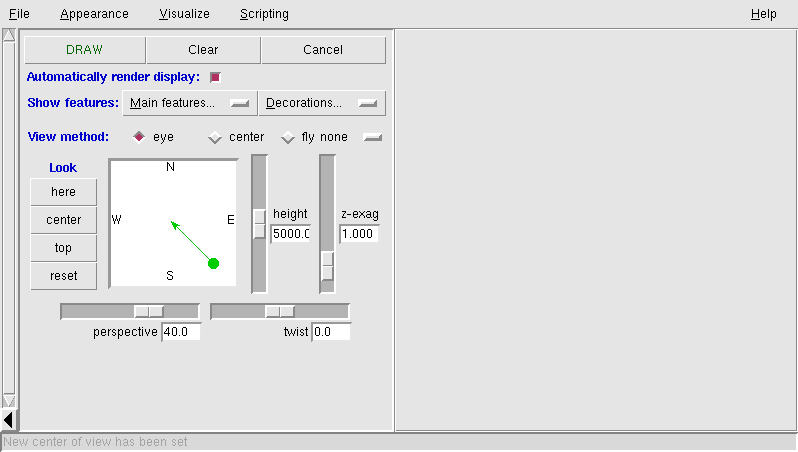
\includegraphics[scale=0.5]{img/screenshot_005}
		\caption{{\small \label{fig:L'interfaccia-principale-di-NVIZ}L'interfaccia principale di NVIZ all'avvio.}}
	\end{figure}
	
	Il programma può essere avviato direttamente dal menù del Layer Manager: \textsf{$\text{File}\rightarrow\text{NVIZ}$}. La finestra che appare a schermo permette di definire alcune opzioni per l'avvio. Se si intende avviare NVIZ senza caricare alcun dato, è sufficiente spuntare l'opzione \textsf{Quickstart - do not load any data} nella scheda \textsf{Optional} e premere \textsf{Run}. Al contrario, se si intende caricare un layer direttamente all'avvio del programma, le schede \textsf{Raster} e \textsf{Vector} consentono di selezionare layer raster per l'elevazione (occorre selezionare il layer SRTM), un eventuale layer raster per i colori o una mappa raster 3D già importata. La scheda \textsf{Vector} consente di selezionare layer di geometrie vettoriali (aree e linee o punti) da sovrapporre al layer 2.5D. Per avviare NVIZ premere \textsf{Run}.

	L'interfaccia di NVIZ (visibile in fig. \ref{fig:L'interfaccia-principale-di-NVIZ}) risulta abbastanza essenziale.

			\paragraph{Punto di vista}
				Il quadrante con i punti cardinali permette, muovendo il pallino, di modificare il punto di vista. Di default la modalità di visualizzazione adottata è la \textsf{eye}, ma è possibile cambiarla in \textsf{fly} per poter accedere alla funzione di esagerazione dell'asse $z$: muovendo infatti la barra di scorrimento verticale \textsf{z-exag} vengono esagerate le dimensioni dell'asse $z$ rispetto agli assi $x$ e $y$, permettendoci di apprezzare meglio la conformazione del territorio.

			\paragraph{Aggiungere decorazioni}
				Il menù \textsf{Decorations} permette di aggiungere decorazioni come la barra di scala, la freccia Nord, la legenda, delle etichette o una frangia, personalizzabili nei dettagli dalle opzioni che appaiono in basso nella finestra.

			\paragraph{Personalizzazioni: la luce}
				Il menù \textsf{Appearence} consente di personalizzare molti aspetti della visualizzazione, come la luce: facendo click sulla voce \textsf{Lighting} appare nell'area di visualizzazione a destra una sfera, colorata secondo la posizione attuale della fonte luminosa; muovendo il puntatore del quadrante apposito presente nelle opzioni per l'illuminazione apparse in basso, è possibile modificare la direzione e la colorazione dlella fonte di luce. Tutte le altre personalizzazioni sono molto intuitive nelle loro impostazioni.

			\paragraph{Aggiungere piani di taglio}
				In situazioni in cui ci siano più layer 2.5D sovrapposti, è utile sezionare il volume visibile con i piani di taglio (\emph{cutting planes} in inglese); possono essere aggiunti attraverso la voce di menù \textsf{$\text{Visualize}\rightarrow\text{Cutting Planes}$} che apre un set di opzioni in basso. Per aggiungere un nuovo piano di taglio, fare click sul pulsante associato ad \textsf{Active cutting plane} e selezionare un piano. Come avviene per il punto di vista o per la fonte luminosa, è possibile sia modificarne la posizione muovendo il cursore sul quadrante di posizionamento sia agendo sui cursori verticali.

			\paragraph{Aggiungere ulteriori layer}
				\begin{figure}
					\centering
					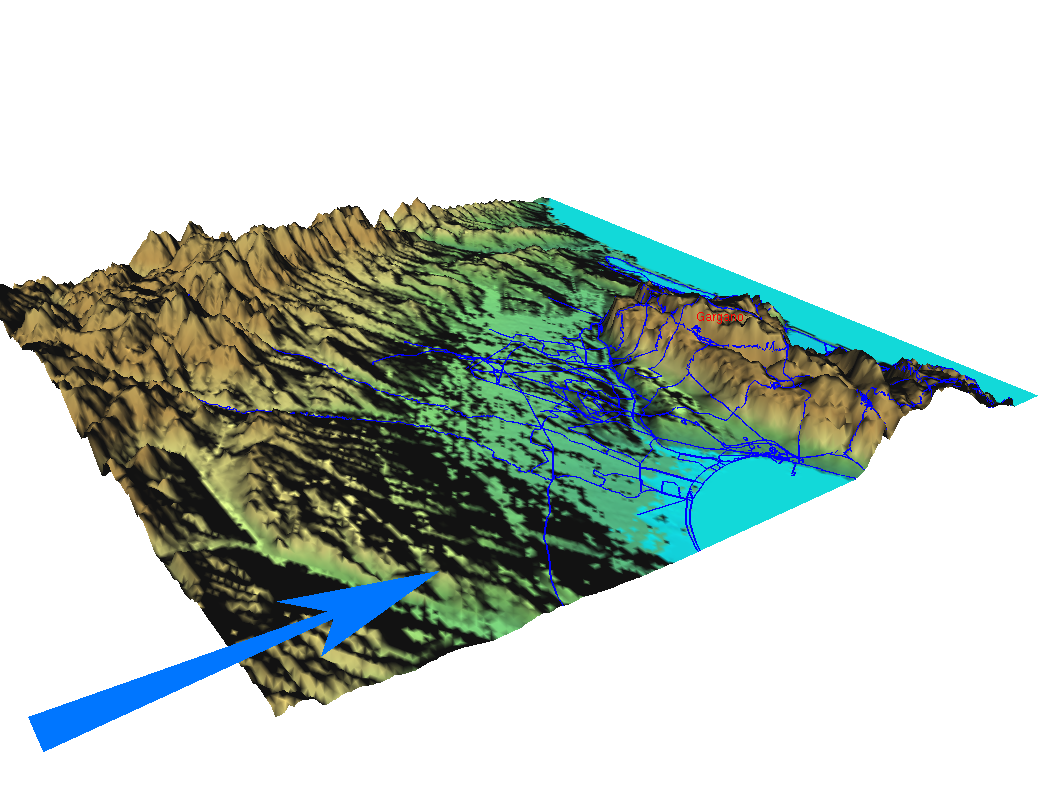
\includegraphics[scale=0.3]{img/prova}
					\caption{{\small Il grafo stradale della zona del Gargano (Puglia) sovrapposto al modello 2.5D da SRTM; il nord è indicato dalla freccia.}}
				\end{figure}
				
				Per aggiungere altri layer raster o vettoriali è sufficiente selezionare \textsf{$\text{Visualize}\rightarrow\text{Vector Lines/3D Polygons}$}e quindi tra le opzioni che compaiono in basso fare click su \textsf{New }per scegliere mapset e mappa vettoriale da caricare; il risultato sarà simile a quello riportato in fig. . Per caricare un layer raster, analogamente, \textsf{$\text{Visualize}\rightarrow\text{Raster surfaces}$}. In entrambi i casi si dispone in basso in ricco set di opzioni per modificare la visualizzazione a proprio piacimento.

\section{DTM da file \emph{.asc}}
	I file con estensione \emph{.asc} sono dei semplici file di testo ASCII contenenti informazioni di tipo raster sulle quote (un esempio è visibile in fig.~\ref{fig:Esempio-asc}). Uno dei problemi legati all'importazione di file raster è che spesso vengono distribuiti (specialmente quando sono ad alta risoluzione) in file di piccole dimensioni, per fare in modo che possano essere facilmente elaborabili. Da ciò nasce la necessità di dover prima importare e poi unire tra loro anche diverse centinaia di file, ognuno dei quali è solo un tassello nel DTM di una zona molto vasta che potrebbe interessarci.
	
	\begin{figure}
		\centering
		\begin{minipage}[t]{0.5\columnwidth}
			\begin{verbatim}
				ncols 485
				nrows 390
				xllcorner 572517,596
				yllcorner 4616572,835
				cellsize 8
				NODATA_value -9999}
				775,7946 775,7089 776,588 777,8846
				779,1224 780,2703 780,6612 780,9045
				781,1004 780,8962 779,9883 778,9046
			\end{verbatim}
		\end{minipage}
		\caption{{\small \label{fig:Esempio-asc}Esempio di un file raster }\emph{\small .asc }{\small aperto con un normale editor di testo.}}
	\end{figure}

	I passaggi riportati nei paragrafi seguenti sono da intendersi come applicati ai file \emph{.asc}, ma con leggeri adattamenti possono essere replicati per qualsiasi tipo di file raster.

	\subsection{Importare in massa file \texttt{.asc}}
		Uno dei vantaggi di GRASS GIS è il notevole grado di automazione a cui si può ricorrere in caso di grandi quantità di dati. Ad esempio, è possibile scrivere script nel linguaggio di programmazione Bash per automatizzare l'importazione di grandi quantità di file raster, in questo caso \texttt{.asc}. Per importare uno o pochi file \texttt{.asc} è sufficiente ricorrere al modulo \textsf{r.in.arc}, raggiungibile anche dal menù \textsf{$\text{File}\rightarrow\text{Import~raster~map}\rightarrow\text{ESRI~ASCII~grid~import}$}. Le azioni proposte di seguito fanno riferimento all'utilizzo dello script \textsf{raster\_tree.sh}, sviluppato da Francesco Massa e Paolo Zatelli, e rilasciato in licenza libera (si veda in merito \textsection\ref{sec:raster_tree.sh}).
		
		\begin{enumerate}
			\item creare il file dello script e nominarlo \textsf{raster\_tree.sh};
			\item copiare il file dello script nella cartella che contiene i file \emph{.asc};
			\item avviare GRASS GIS nella location in cui si desidera importare i raster\footnote{Si noti bene che non tutti i raster forniti sono già georeferenziati; prima di procedere all'importazione automatica assicurarsi (importando un solo file, che si potrà poi cancellare) che tipo di sistema di riferimento usano i raster, e creare di conseguenza la location adatta in cui importarli. In futurò sarà sempre possibile importarli in un altro sistema di riferimento, riproiettandoli.};
			\item dal terminale di GRASS, posizionarsi nella cartella contenente i raster e lo script ed avviare quest'ultimo con il comando

			\texttt{./raster\_tree.sh}

		\end{enumerate}
		
		Al termine, lo script avrà importato tutti i raster all'interno della location nella quale ci si è posizionati all'avvio. Infatti, caricando un nuovo layer raster, nell'elenco dovrebbero apparire anche i raster di recente importazione.

		\input{tab/box_importare_diversi_raster}

	\subsection{Unire più \emph{.asc} in un unico raster}
		Una volta importati tutti i file raster che compongono il DTM della zona in analisi, si è ottenuto un mosaico di immagini, ma niente più di questo. Il passo successivo consiste appunto nell'unire tale mosaico in un'unica immagine, tramite il modulo r.patch, la cui interfaccia grafica è avviabile usando l'omonimo comando dal terminale di GRASS.  In questo caso, nel campo Name of raster maps to be patched together occorrerà selezionare una ad una tutte le mappe; nel caso si debbano unire 50 file raster, l'utilizzo dell'interfaccia grafica diventa inefficiente, laddove da terminale sono sufficienti pochi comandi per portare a termine l'operazione, vediamo come\footnote{I comandi che seguono partono dal presupposto che i raster del DTM siano stati scaricati da un sistema automatizzato (ad esempio un SIT online, un webgis e simili) e che ogni file abbia nel proprio nome, come accade sempre in questi casi, un prefisso standard seguito dalle informazioni sulla zona geografica alla quale si riferisce, ad esempio: \texttt{g\_43a64b}.}:
		
		\begin{enumerate}
			\item avviare GRASS e dal terminale posizionarsi nella location che contiene i file raster;
			\item dare i seguenti comandi:

			\begin{verbatim}
				MAPS=`g.mlist type=rast sep=, pat=``g_{*}''`
				g.region rast=\$MAPS
				r.patch in=$MAPS out=DTM_unito
			\end{verbatim}
		\end{enumerate}
		
		Analizziamone il significato:
		
		\begin{description}
			\item [{\texttt{MAPS=}}] viene definita una variabile di nome \texttt{MAPS}, ovvero viene assegnata ad una parte della memoria disponibile sul computer un certo valore, che è definito in base ai comandi che si trovano dopo il simbolo \texttt{=}, e compreso tra i due apici ``\texttt{ `}''\footnote{In fase di definizione della variabile, gli apici vengono ottenuti con la combinazione di tasti \textsf{AltGr+'}.}.
			\item [{\texttt{g.mlist}}] è il comando che elenca tutte le tipologie di file presenti nella location; i file da elencare vengono ``scremati'' in base agli attributi elencati di seguito a \texttt{g.mlist}, in questo caso
				
				\begin{description}
					\item [{\texttt{type=rast}}] elenca solo i file raster; alternativamente, può assumere anche valore \texttt{vect};
					\item [{\texttt{sep=,}}] questo attributo specifica quale separatore di file deve essere usato all'interno dell'elenco, in questo caso una virgola;
					\item [{\texttt{pat=g\_{*}}}] elenca solo i file che rispettano un certo \emph{pattern}, ovvero che hanno nel proprio nome il prefisso definito, in questo caso \texttt{g\_{*}}; l'asterisco indica la fine del prefisso e l'inizio di una parte del nome del file che può variare a seconda del file.
				\end{description}
		\end{description}
		
		Il risultato del comando \texttt{g.mlist type=rast sep=, pat=``g\_{*}''} è il seguente elenco:
		
		\begin{verbatim}
			g_397072,g_397102,g_397111,g_397112,g_397113,g_397114,g_397123,g_397141, ...
		\end{verbatim}
		
		È chiaramente visibile che l'elenco generato riporta tutti i file raster il cui nome inizia per ``\texttt{g\_}'', separati da una virgola. Tutto questo elenco viene quindi attribuito alla variabile \texttt{MAPS}, che viene poi utilizzata nel comando successivo per impostare la region; è importante infatti che prima che le mappe raster vengano unite, la region in cui si sta lavorando (che era stata prima appositamente creata allo scopo) venga ridimensionata a misura esatta del file raster che si otterrà dopo l'unione. Il comando \texttt{g.region rast=\$MAPS} ridimensiona la region in base alla somma delle estensioni delle mappe all'interno della variabile \texttt{MAPS}.

		Il terzo e ultimo comando avvia il modulo \texttt{r.patch} per procedere all'unione effettiva di tutti i raster di input (elencati nella variabile \texttt{MAPS}) in un unico file di output, a cui è stato dato nome \texttt{DTM\_unito}. Occorre notare a questo punto che il raster ottenuto potrebbe non essere necessariamente georeferenziato, e bisognerà procedere come descritto precedentemente per la georeferenziazione (o riproiezione, se già georeferenziato ma in un differente sistema di riferimento; rispettivamente \textsection\ref{sec:Georeferenziare-una-carta-raster} e \ref{sec:Riproiettare-raster}) di un raster.
